%!TEX root = ./nips_2018_sketchmcmc_supp.tex



\section{Additional Experimental Results}

In Figures~\ref{fig:suppmnist} and \ref{fig:suppfmnist} below, we provide the evolution of the SWF algorithm on the Fashion MNIST and the MNIST datasets in higher resolution.

\newcommand{\picwidth}{0.15}%originally 0.24

\begin{figure}
\centering
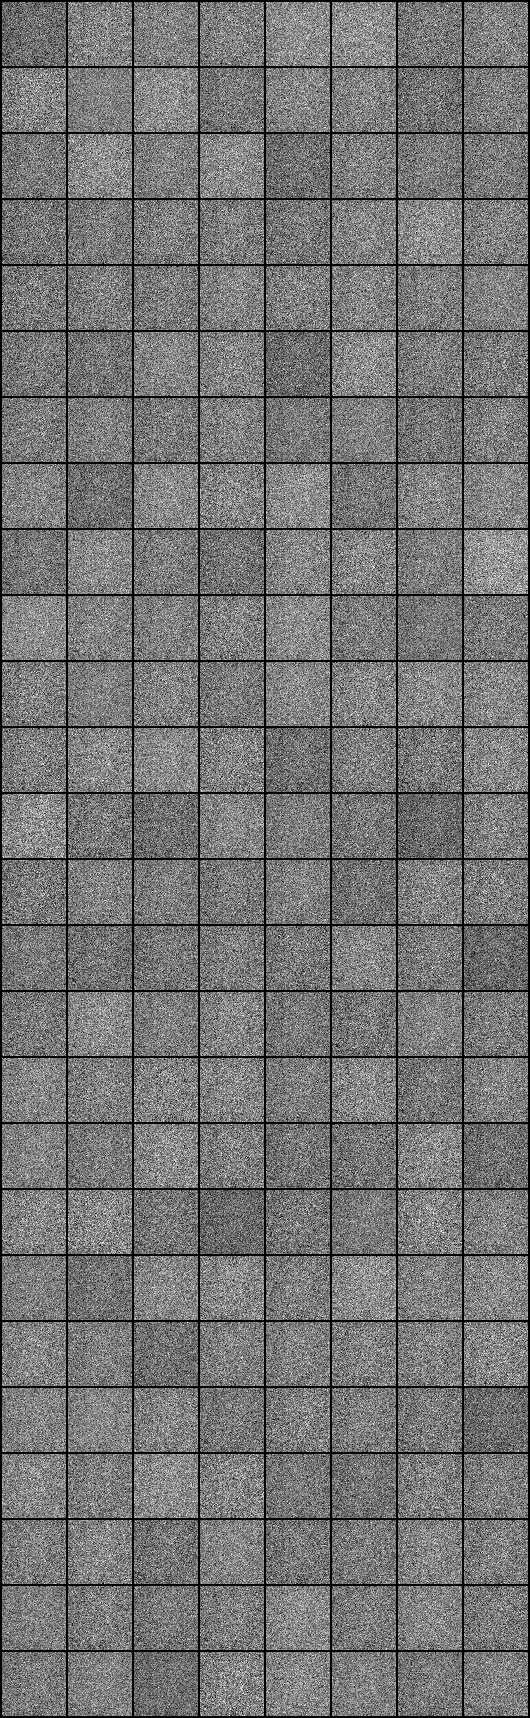
\includegraphics[width=\picwidth\columnwidth]{supplementary/mnist/image_0.png}
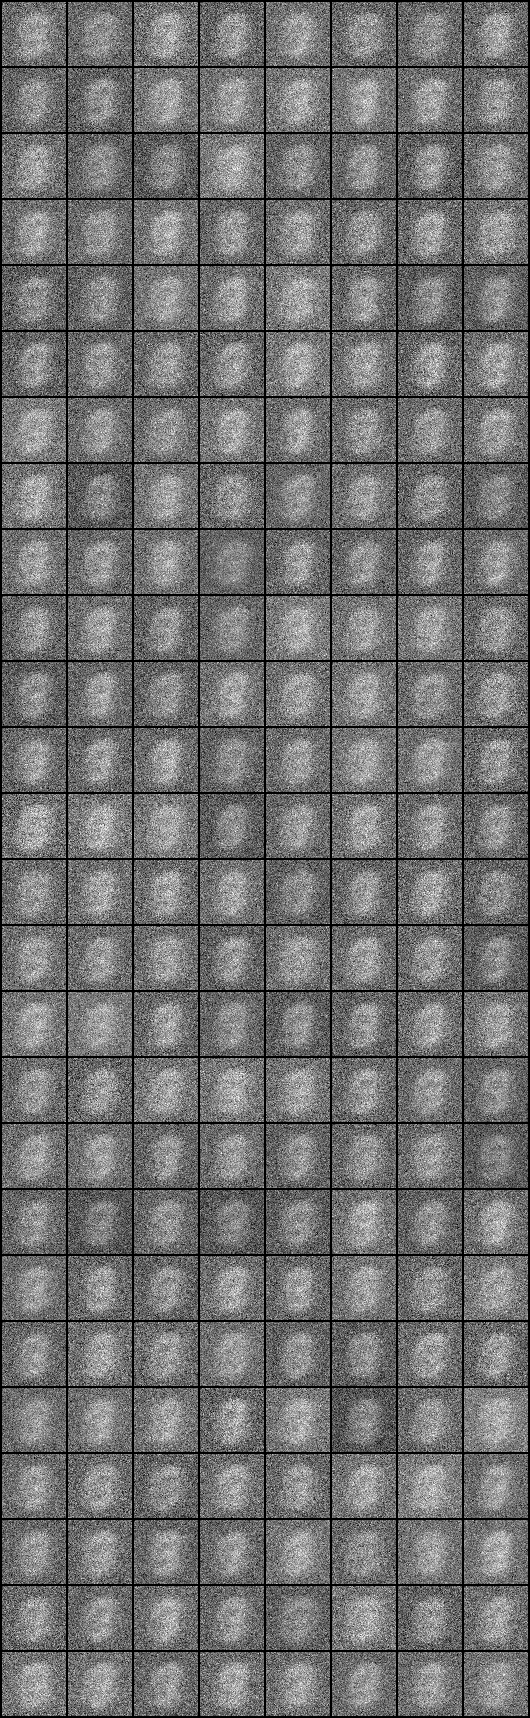
\includegraphics[width=\picwidth\columnwidth]{supplementary/mnist/image_50.png}
\includegraphics[width=\picwidth\columnwidth]{supplementary/mnist/image_100.png}
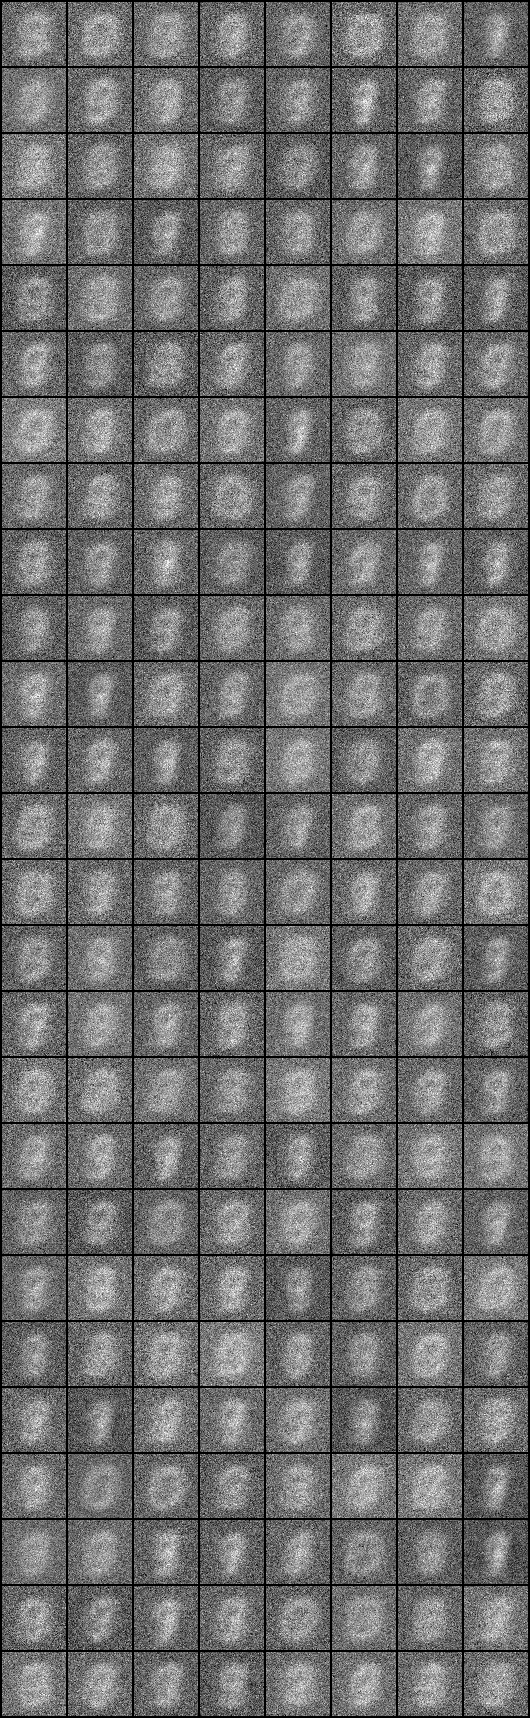
\includegraphics[width=\picwidth\columnwidth]{supplementary/mnist/image_200.png}\\
\includegraphics[width=\picwidth\columnwidth]{supplementary/mnist/image_500.png}
\includegraphics[width=\picwidth\columnwidth]{supplementary/mnist/image_1000.png}
\includegraphics[width=\picwidth\columnwidth]{supplementary/mnist/image_5000.png}
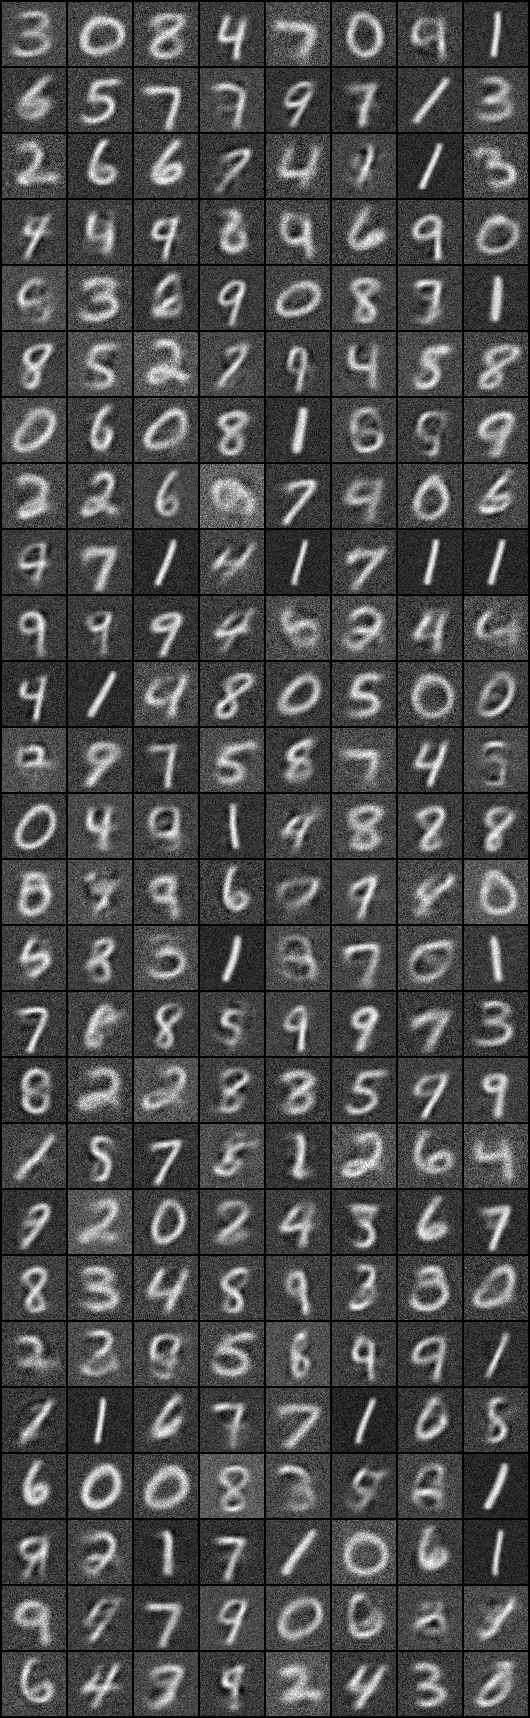
\includegraphics[width=\picwidth\columnwidth]{supplementary/mnist/image_25000.png}
\caption{The evolution of SWF through 15000 iterations on the MNIST dataset.}
\label{fig:suppmnist}
\end{figure}

\begin{figure}
\centering
\includegraphics[width=\picwidth\columnwidth]{supplementary/alternative_fmnist/image_100.png}
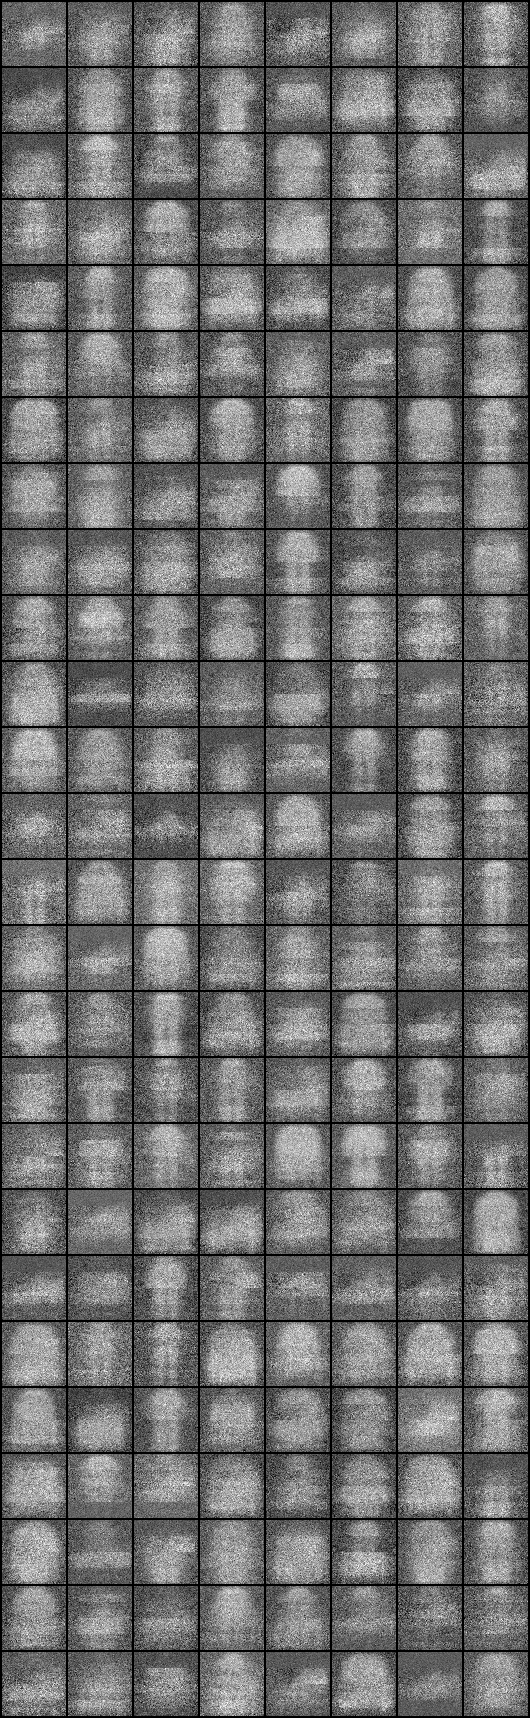
\includegraphics[width=\picwidth\columnwidth]{supplementary/alternative_fmnist/image_250.png}
\includegraphics[width=\picwidth\columnwidth]{supplementary/alternative_fmnist/image_500.png}
\includegraphics[width=\picwidth\columnwidth]{supplementary/alternative_fmnist/image_1000.png}\\
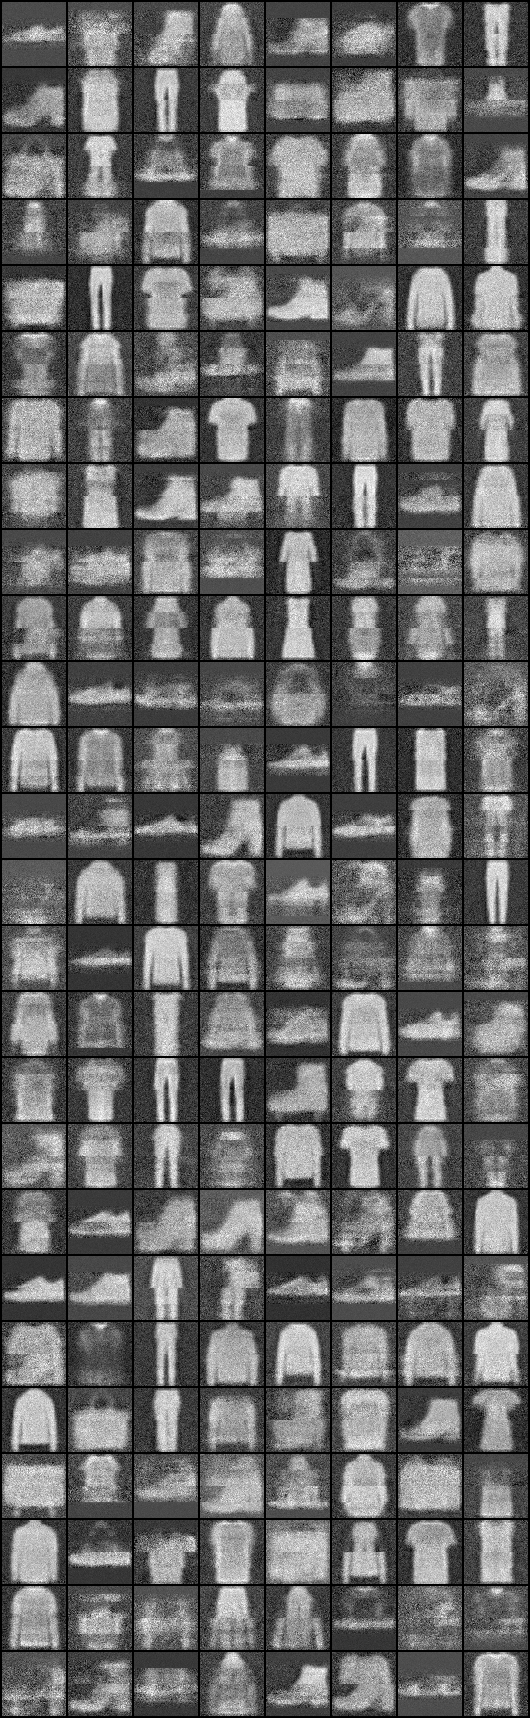
\includegraphics[width=\picwidth\columnwidth]{supplementary/alternative_fmnist/image_2000.png}
\includegraphics[width=\picwidth\columnwidth]{supplementary/alternative_fmnist/image_5000.png}
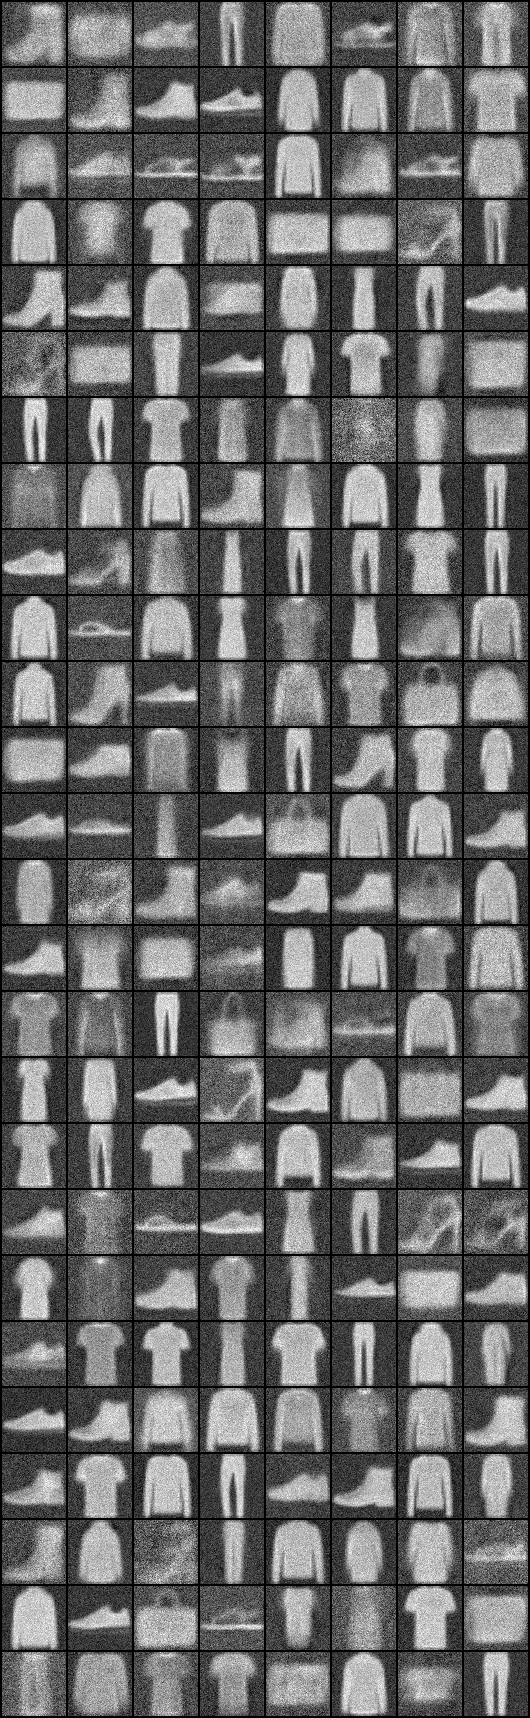
\includegraphics[width=\picwidth\columnwidth]{supplementary/alternative_fmnist/image_10000.png}
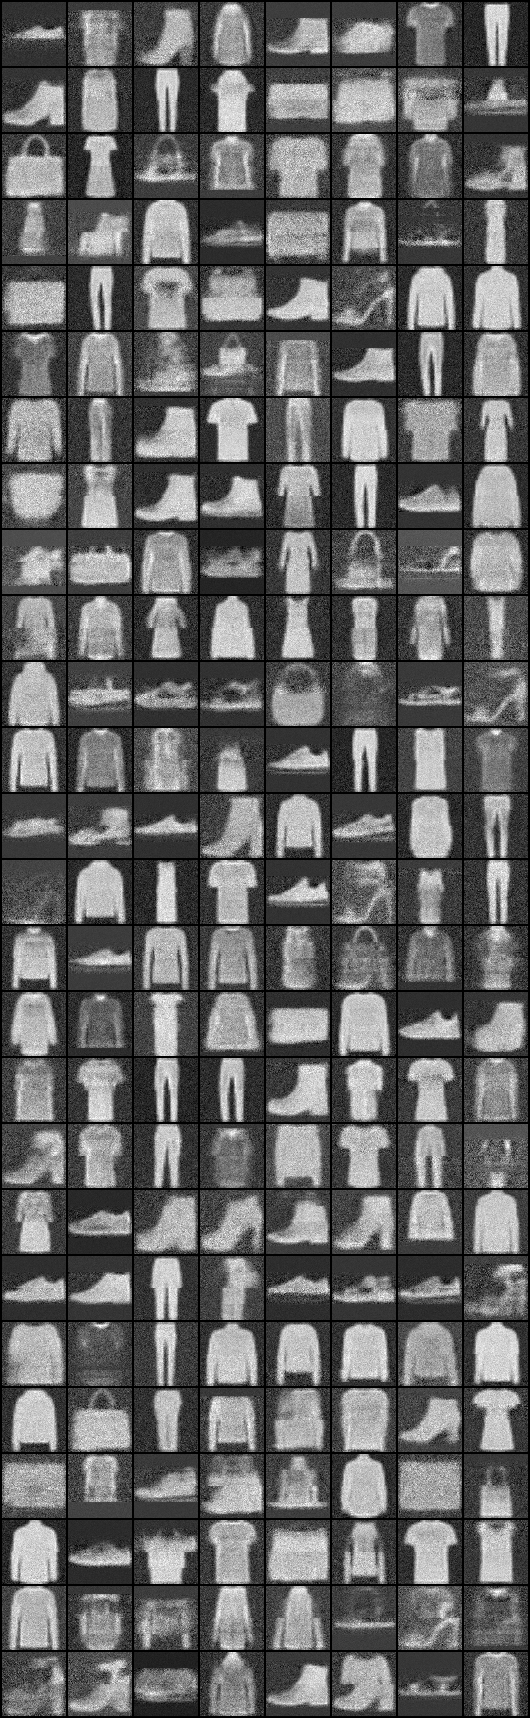
\includegraphics[width=\picwidth\columnwidth]{supplementary/alternative_fmnist/image_15000.png}
\caption{The evolution of SWF through 15000 iterations on the Fashion MNIST dataset.}
\label{fig:suppfmnist}
\end{figure}







% \section{Details of Computing $(F_{\theta_{n}^*\#\hat{\mu}}^{-1} \circ F_{\theta^*_{n}\#\nu}) $}


% \umut{Antoine. -- sorting, interpolation etc}

% \begin{figure}
% \begin{centering}
% \setlength\tabcolsep{1pt}
% \begin{tabular}{cccccc}
% $\lambda=0$ & $\lambda=0.1$ & $\lambda=0.2$ & $\lambda=0.3$ & $\lambda=0.5$ & $\lambda=1$\tabularnewline
% 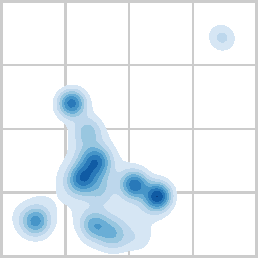
\includegraphics[width=2cm]{figures/supplementary/regularization/r0_output_dist_k=70-crop.pdf} & 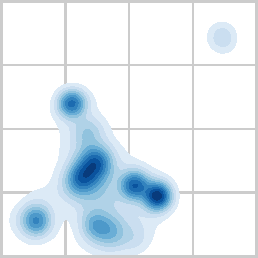
\includegraphics[width=2cm]{figures/supplementary/regularization/r01_output_dist_k=70-crop.pdf} & 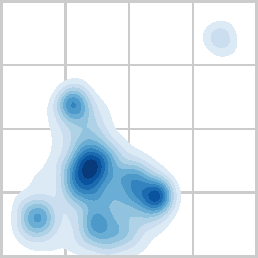
\includegraphics[width=2cm]{figures/supplementary/regularization/r02_output_dist_k=70-crop.pdf} &  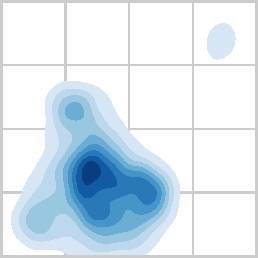
\includegraphics[width=2cm]{figures/supplementary/regularization/r03_output_dist_k=70-crop.pdf}&  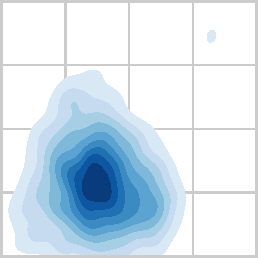
\includegraphics[width=2cm]{figures/supplementary/regularization/r05_output_dist_k=70-crop.pdf} &  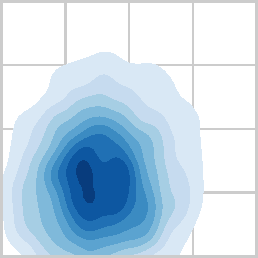
\includegraphics[width=2cm]{figures/supplementary/regularization/r1_output_dist_k=70-crop.pdf}
% \end{tabular}
% \par\end{centering}
% \caption{Influence of the regularization parameter $\lambda$. The higher $\lambda$, the more entropic the output distribution.\label{fig:lambda_supp}}
% \end{figure}
